\documentclass{beamer}

% Configuración para mostrar números en la tabla de contenidos
\setbeamertemplate{section in toc}[sections numbered]
\usetheme{Frankfurt}
\usepackage{graphicx}
\renewcommand{\normalsize}{\fontsize{7}{5}\selectfont} 

\title{Automatización del proceso de evaluación en exámenes de opción múltiple, un enfoque para optimizar la calificación y el registro de notas}
\author{Michael Santiago Jiménez Caballero}
\date{\today}


\begin{document} %_____________________________________**__________________________________

\frame{\titlepage}
\begin{frame}{Contenido}
    \tableofcontents
\end{frame}

\section{Resumen}
\begin{frame}{Resumen}
    En el presente documento se muestra el desarrollo de una aplicación web que automatiza la  calificación de exámenes de
    opción múltiple mediante redes neuronales convolucionales y  algoritmos de 
    reconocimiento óptico de caracteres. La implementación incluye una aplicación
    web y logra un 97\% de precisión, optimizando el proceso de evaluación y los recursos docentes.
\end{frame}

\section{Introducción}
\begin{frame}{Introducción}
    Se resalta la necesidad de automatizar la calificación de exámenes de opción múltiple en Colombia para reducir 
    la carga de los docentes y mejorar el enfoque en la enseñanza. Las limitaciones tecnológicas y el predominio 
    de métodos tradicionales, como el examen ICFES, refuerzan esta necesidad. Se propone un sistema de 
    calificación automática basado en OCR y dispositivos sencillos, como smartphones, para agilizar el 
    proceso y optimizar el tiempo dedicado a actividades pedagógicas.    
\end{frame}

\section{Problema}
\begin{frame}{Problema}
    Este proyecto destaca la importancia de automatizar la calificación en la educación básica, ofreciendo 
    una solución para optimizar el trabajo de los docentes en la evaluación de pruebas. Actualmente, 
    la calificación manual consume recursos significativos, limitando el enfoque en el aprendizaje. 
    La automatización no solo reduce este trabajo, también genera estadísticas descriptivas clave 
    sobre el desempeño estudiantil, facilitando decisiones pedagógicas más informadas, incluso en
     contextos con acceso tecnológico limitado.
\end{frame}

\section{Justificación}
\begin{frame}{Justficación}
    \begin{itemize}
        \item Se  plantea que el desarrollo de una aplicación que automatice la calificación de exámenes de selección múltiple, utilizando visión artificial.  puede permitir que el sistema obtenga una alta precisión, optimizando el trabajo docente y permitiendo el uso de recursos accesibles como smartphones. 
        \item Además, de agilizar la calificación, el proyecto promueve un equilibrio entre las tareas administrativas y pedagógicas, liberando recursos para mejorar la calidad del aprendizaje. Esta innovación responde a los desafíos actuales en la educación básica colombiana, destacando el impacto positivo de la automatización en el proceso educativo
    \end{itemize}
\end{frame}

\section{Objetivo General}
\begin{frame}{Objetivo General}
    \begin{itemize}
        \item Desarrollar un modelo de visión artificial para automatizar la calificación de exámenes de selección múltiple mediante algoritmos de reconocimiento óptico de caracteres, con el fin de reducir la carga laboral de los docentes.
    \end{itemize}
\end{frame}

\section{Objetivos Específicos}
\begin{frame}{Objetivos Específicos}
    \begin{itemize}
        \item Realizar funciones de preprocesamiento de las imágenes para la limpieza de estas.
        \item Implementar un algoritmo de Reconocimiento Óptico de Caracteres (OCR) para encontrar patrones en las imágenes, permitiendo la extracción automática de las respuestas seleccionadas por los estudiantes.
        \item Realizar un modelo que utilice redes neuronales convolucionales para la clasificación de múltiples clases.
        \item Desarrollar funciones vinculen el algoritmo de OCR con el modelo y permita reconocer como las opciones seleccionadas por cada estudiante, y las organice para su evaluación.
        \item Realizar pruebas exhaustivas del algoritmo OCR en diferentes tipos de hojas de respuestas, garantizando una precisión superior al 90\% en la detección de las respuestas.
        \item Desplegar los algoritmos en una aplicación web
    \end{itemize}
\end{frame}

\section{Antecedentes}
\begin{frame}{Antecedentes}
    \textbf{Sistema de Puntuación Automatizado para Exámenes de Opción Múltiple con Retroalimentación Rápida}
    \begin{itemize}
        \item Este proyecto se basa en el trabajo de Chai \& Alomran (2018), quienes utilizaron procesamiento de imágenes y OCR para automatizar la calificación de exámenes de opción múltiple.
        \item Su tecnología identifica respuestas manuscritas sin necesidad de formularios costosos ni equipos especializados.
        \item Mediante técnicas avanzadas de OCR, el sistema procesa hojas escaneadas, reconoce códigos de identificación y detecta las respuestas seleccionadas con alta precisión.
        \item Este modelo resalta que la automatización de la puntuación es eficiente, accesible y representa un avance importante en la mejora de los procesos educativos.
    \end{itemize}
\end{frame}

\begin{frame}{Antecedentes}
    \textbf{Android Based Automated Scoring of Multiple-Choice Test}
    \begin{itemize}
        \item Este proyecto propone una solución accesible y económica para automatizar la calificación de exámenes de opción múltiple, utilizando tecnologías como OCR y procesamiento de imágenes.
        \item Se emplean teléfonos inteligentes Android para reemplazar los lectores ópticos tradicionales, mejorando la accesibilidad en contextos con recursos limitados.
        \item El sistema detecta marcas de "X" en hojas de respuestas y alcanza un reconocimiento del 90\%, optimizando la evaluación educativa y reduciendo costos.
        \item Este enfoque es práctico y eficiente, adaptado a las necesidades actuales del ámbito educativo.
    \end{itemize}
\end{frame}

\section{Marco Teórico}
\begin{frame}{Marco Teórico}
    Los algoritmos de OCR permiten extraer información importante de las imágenes a través de diferentes parámetros, una vez se establecen es posible la recolección de información, la cual, se puede utilizar en un modelo de redes neuronales convolucionales (CNN), que se encargan de de claisificar de acuerdo con los diferentes mapas de características,
    pasando por diferentes procesos como la construcción del modelo utilizando CNN, construcción del algoritmo de reconocimiento óptico de caracteres
\end{frame}


\begin{frame}{Redes neuronales convolucionales CNN}
    Las redes neuronales convolucionales (CNN), también conocidas como ConvNets, son un tipo especializado de arquitectura de redes neuronales profundas diseñadas específicamente para procesar datos de imágenes. Estas redes son altamente efectivas en tareas de visión por computadora, incluido el reconocimiento de patrones y la clasificación de objetos. El momento el que las CNN se posicionan como una tecnología especializada en el análisis de imágenes, fue en el 2010 con la competencia anual de ImageNet, en la cual, se utiliza este mismo conjunto de datos que posee cerca de quince millones de imágenes clasificadas en veinte mil categorías. A partir de este punto, las CNN se reconocen principalmente por su desempeño significativamente alto, la relativa disminución del tiempo de entrenamiento en relación con los diferentes modelos y el uso de tarjetas gráficas para procesar las imágenes (Krizhevsky, Sutskever, \& Hinton, 2012). La arquitectura de una CNN se basa en el concepto de convolución, que es una operación matemática fundamental en el procesamiento de señales.
\end{frame}


\subsection{Convolución}
\begin{frame}{Convolución}
    La convolución transforma datos de entrada, como imágenes, utilizando filtros llamados "Kernels" que extraen características. Matemáticamente, el resultado de la convolución se expresa como:
    \[
        S(i,j) = \sum\sum I(i + m, j + n) \cdot K(m, n)
    \]
    El Kernel recorre la imagen realizando un producto punto entre la imagen y el filtro, generando un "mapa de características". Este proceso consume muchos recursos, por lo que se recomienda usar capas de Pooling para optimizar el entrenamiento (Seiler \& Fergus, 2014).
    \begin{figure}
        \centering
        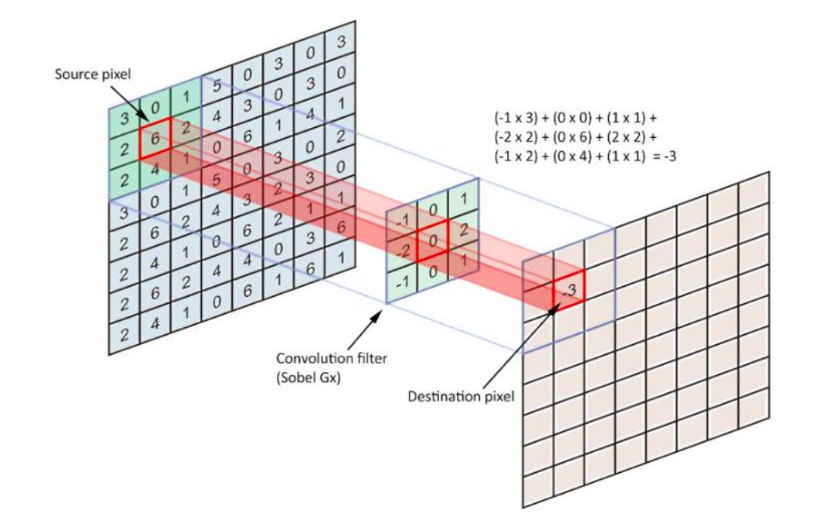
\includegraphics[width=0.5\textwidth]{/home/lic-jimenez/Documents/Tesis-Final/Slides/conv_1.png}
        
    \end{figure}
\end{frame}



\subsection{Pooling}
\begin{frame}{Pooling}
    \begin{itemize}
        \item La principal función de las capas pooling es reducir la dimensionalidad entre el conjunto de datos con las representaciones hechas por el Kernel, de forma que se disminuye el tamaño de la matriz de salida, permitiendo que se retengan las características sobresalientes del conjunto de datos de entrada y depurando aquellas como el ruido que no aportan información relevante.   
        \item El tipo más común es Max Pooling, que se aplica de forma semejante a la del Kernel, es decir, utilizando matrices de 2*2 o 3*3, selecciona los píxeles con mayor intensidad en la escala de grises y lo pasa a una nueva matriz, por otra parte, aquellos con menor intensidad son despreciados. De esta forma, se reduce significativamente la dimensionalidad de los mapas de características, sin perder información relevante.     
    \end{itemize}

    \begin{figure}
        \centering
        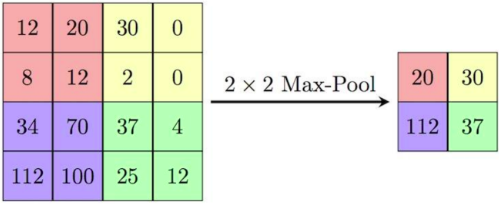
\includegraphics[width=0.5\textwidth]{/home/lic-jimenez/Documents/Tesis-Final/Slides/pool_1.png}
    \end{figure}
\end{frame}


\subsection{ReLU}
\begin{frame}{ReLU}
    Diversos autores sugieren que se puede aplicar la función ReLU luego de las capas de Pooling, teniendo en cuenta que en éstas los objetos ya se encuentran lo suficientemente caracterizados con las dimensiones reducidas, ahora a cada elemento de las marices es sometido en la siguiente función:
    
    \[
    f(x) = max (0, x)
    \]

    Implicando unas consideraciones iniciales a la hora de utilizar esta función de activación, estas son, el poco consumo de recursos computacionales ya que evalúa los elementos de las matrices y si son menores o iguales que cero, se obtiene un 0 en la posición de ese elemento, si por el contrario es mayor que cero, obtendrá el valor de intensidad correspondiente. Es decir, el uso de la función ReLU permite que los valores positivos pasen a la siguiente capa sin cambios y los negativos sean convertidos en 0. Lo anterior plantea una no linealidad, permitiendo que en el entrenamiento el modelo pueda aprender relaciones complejas, no obstante, el uso de esta función de activación plantea un problema y es que es vulnerable a convertir tantos elementos en cero que podrían apagarse algunas neuronas indefinidamente, o como se conoce neurona muerta.

\end{frame}


\subsection{Capas Flatten}
\begin{frame}{Capas Flatten}
    Al tener un mapa de características robusto se aplica una capa en la que se deben “aplanar” las dimensiones, es decir, si se utiliza imágenes en escala de grises, se puede afirmar que solamente se están utilizando dos dimensiones para la altura y el ancho, a estas se le adiciona la tercera dimensión que corresponde a las diferentes tonalidades (entre blanco y negro) que puede tomar cada pixel, sin embargo, es necesario pasar del tensor mencionado anteriormente a un vector con una única dimensión (con la multiplicación de las dimensiones de cada matriz como la longitud del vector). Permitiendo que la información de la imagen se pueda utilizar en capas completamente conectadas y sobre éstas se pueda hacer la clasificación o predicción
\end{frame}


\subsection{Capas Dense}
\begin{frame}{Capas Dense}
    Las capas Dense o fully conected, se encargan de conectar cada una de las neuronas generadas por las capas Flatten con el fin de que en las últimas etapas del proceso de aprendizaje, el modelo pueda evaluar las características de cada una de las clases y diferenciarlas. Permitiendo que el modelo pueda caracterizar aún más cada uno de los elementos que procesa esta capa. Considerando que, el vector unidimensional generado en la capa Flatten posee diferentes elementos que hacen referencia a una clase, es decir, cada elemento da razón de los mapas de características aplicados y se guarda un patrón de información respectivo, esta información es la que permite conocer cómo las clases se relacionan entre sí y que el modelo pueda determinar a qué clase pertenece.     
\end{frame}



\subsection{Función Softmax}
\begin{frame}{Función Softmax}  
   El uso de la función Softmax es ideal para problemas de clasificación multiclase y teniendo en cuenta que en el proyecto se utilizaron alrededor de 36 clases es posible utilizar la función de activación softmax, esto se debe a que dado un vector unidimensional (proporcionado por la capa Flatten) se pueda evaluar la probabilidad que tiene un elemento del vector a pertenecer a una clase
    \[
   softmax(z_i) = \frac{e^{z_i}}{\sum_j e^{z_j}}
    \]
    Siendo Z el vector, i la clase a la que pertenece y j hace referencias a los diferentes mapas de características, teniendo en cuenta que para cada mapa se evalúa la probabilidad desde 0 hasta 1, donde los valores cercanos a cero muestran que no hay una correspondencia con la clase que se evalúa, por otro lado, aquellos que se aproximan al uno son los que tienen mayor probabilidad de que puedan pertenecer a determinada clase. De esta forma es como se pasa de un vector unidimensional a conocer la probabilidad que tiene una clase de pertenecer a un mapa de características.
    
\end{frame}


\subsection{Estructura de la red}
\begin{frame}{Estructura de la red}
    \begin{figure}
        \centering
        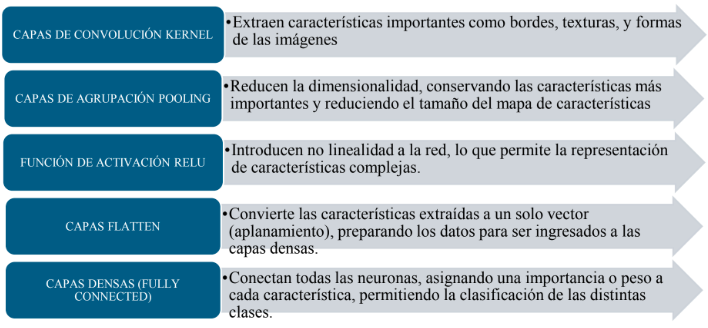
\includegraphics[width=1\textwidth]{/home/lic-jimenez/Documents/Tesis-Final/Slides/resume_1.png}
    \end{figure}
\end{frame}


\subsection{Sistema de calificación}
\begin{frame}{Sistema de calificación}
    \begin{itemize}
        \item \textbf{Accuracy}: También conocido como precisión, es la proporción de las diferentes clases identificadas correcta o incorrectamente (usualmente se utiliza de forma aprobatoria), entre el total de imágenes predichas, obteniendo un resultado entre 0 y 1, donde los valores cercanos a 1 muestran que el modelo reconoce satisfactoriamente las imágenes, por otra parte, cuando se aproxima a 0 da razón de una mala identificación.    
        \[
        Accuracy = \frac{True predictions}{Total predictions}
        \]
        \item \textbf{Recall}: Está dado por aquellas predicciones realizadas por el modelo en las imágenes tanto de entrenamiento como de validación, en las que evalúa los verdaderos positivos entre la suma de los verdaderos positivos y los falsos negativos
        \item \textbf{F1-score}: Se puede considerar el f1-score como el punto medio entre el Accuracy y Recall, dado que evalúa tanto los verdaderos positivos, falsos negativos y los correctamente identificados
    \end{itemize}
\end{frame}


\section{Metodología}
\begin{frame}{Metodología}
    \begin{itemize}
        \item Considerando que el punto central de este trabajo es el desarrollo e implementación de un sistema de
        automatización para la calificación de exámenes de opción múltiple, se determina que el enfoque
        metodológico para la investigación será cuantitativo, usando un diseño transeccional predictivo.
    \end{itemize}    
\end{frame}


\section{Discusión y conclusiones}
\begin{frame}{Discusión y conclusiones}
    \begin{itemize}
        \item En este tr

    \end{itemize}
\end{frame}













\end{document}
